\section{评估实践与证据成熟度}
\subsection{针对具体主张的证据类型}

L0--L5 记录主张如何得到支持：概念、分析、仿真/数据、原型、现场试验和持续运行。图~\ref{fig:maturity} 将每种证据形式与其输入、推理或评估，以及输出相联系。形式上的正确性、实验控制、环境代表性和运行持续时间，仍是相互独立的评估维度。

\begin{figure}[!htbp]\centering
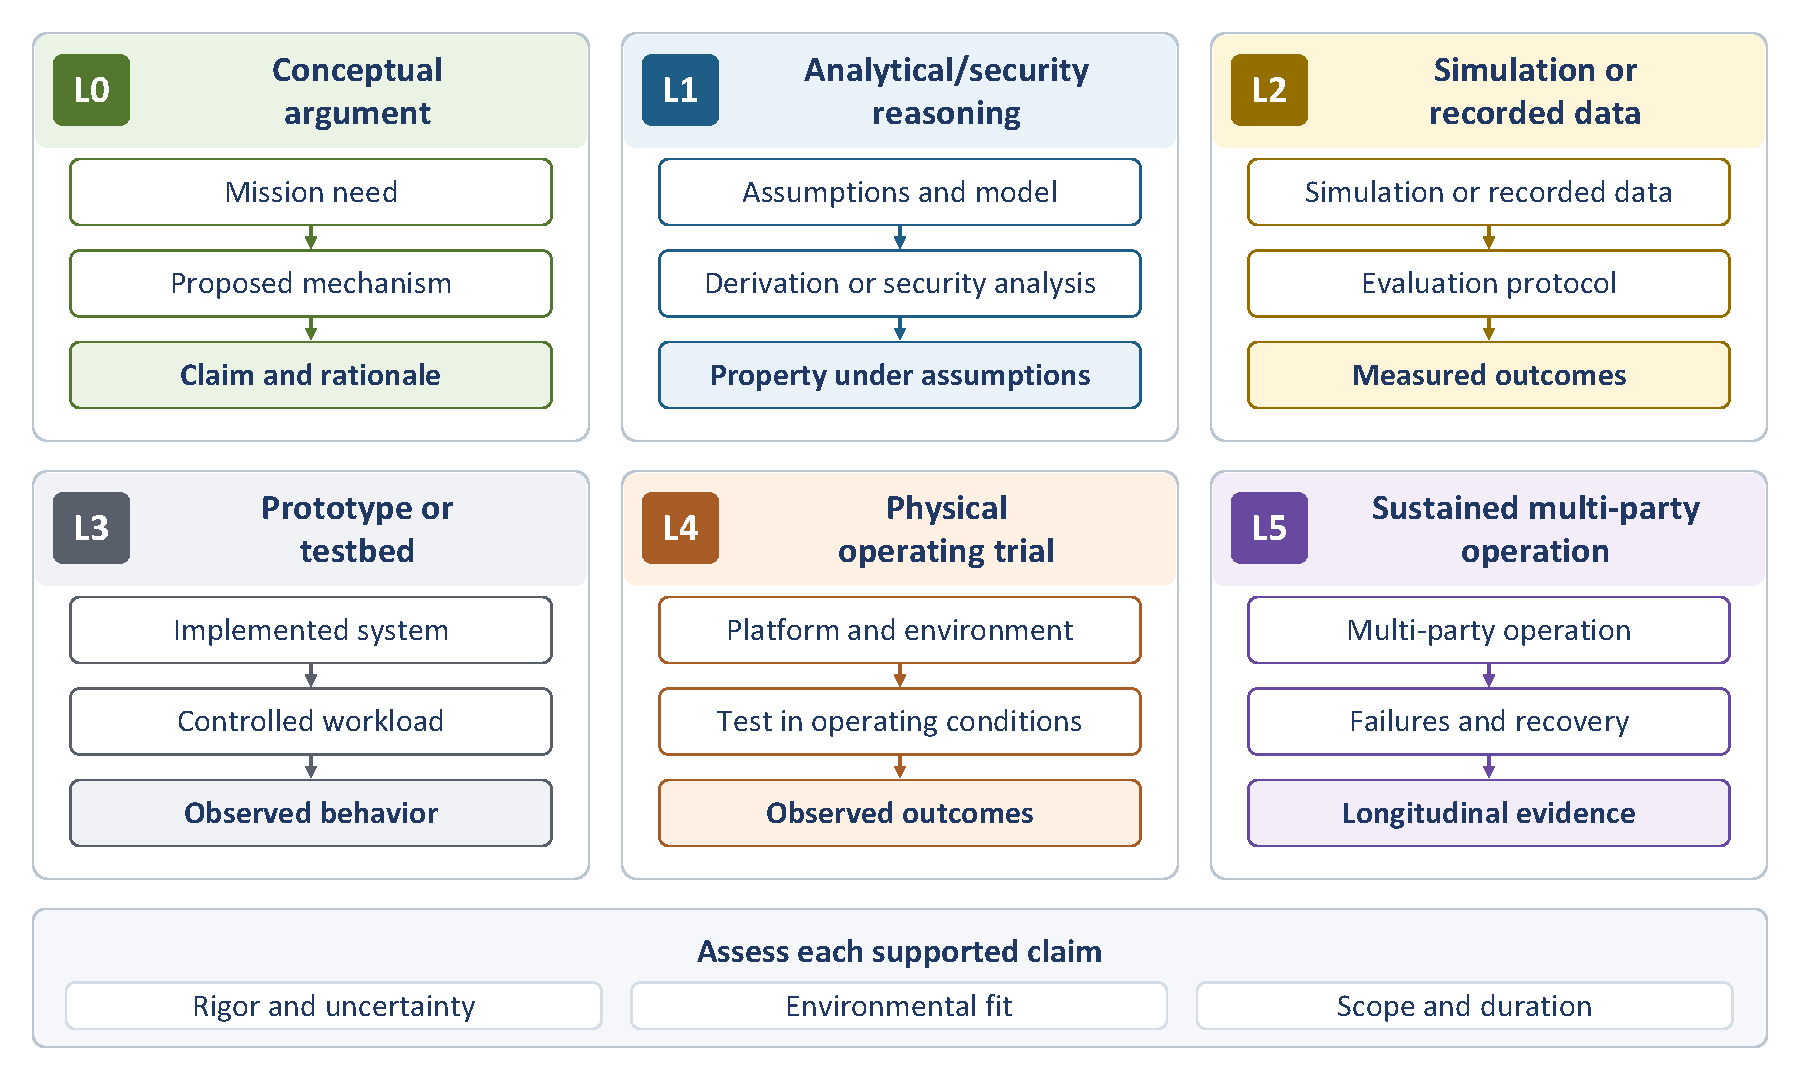
\includegraphics[width=\textwidth]{figures/figure-07-evidence-maturity.pdf}
\caption{互补的证据形式及其对具体主张的支持。各面板连接输入、推理或评估，以及输出；严谨性、环境适合性和范围分别评估。}\label{fig:maturity}
\end{figure}

在 39 项研究样本中，6 项的证据类型包含 L0，11 项包含 L1，20 项包含 L2，20 项包含 L3，1 项包含 L4；没有研究包含 L5。类型存在重叠；4 项研究仅有概念证据。L4 归类针对 S31 限定范围的实体 UAV 节点协作/路由实验；其容器共识基准测试仍为 L3。第~\ref{sec:sensitivity} 节将仅把该实验归为 L3 作为敏感性变体进行评估。BUS 提供硬件原型证据，而记录的 GNSS 轨迹支持 L2。这些环境回答有关实现、实体运行和迁移的不同问题。

如第~\ref{sec:comparative} 节的比较所示，证据形式、参数强度、实际测试的机制和环境相关性，共同决定所支持的主张。

\subsection{数据集、仿真器与试验台}

公共资源支持互补的评估任务。CICIoT2023、TON\_IoT 和 Edge-IIoTset 提供攻击与遥测数据，用于分类和鲁棒性测试\citep{neto2023ciciot2023,alsaedi2020ton,ferrag2022edge}。SeaDronesSee 提供海事视觉数据\citep{varga2022seadronessee}。AirSim、UUV Simulator 和 Aqua-Sim NG 分别面向载具/传感器仿真、水下动力学和水下通信\citep{shah2018airsim,manhaes2016uuv,martin2017aqua}。在同一实验中使用它们，需要兼容的时钟、几何、运动性和事件接口，并配套经过独立验证的任务损失模型。表~\ref{tab:evaluation} 汇总这些资源和迁移检查。

\begin{table}[H]\small
\caption{评估资源与所需的迁移检查。}\label{tab:evaluation}
\begin{tabularx}{\textwidth}{LLL}\toprule
\textbf{资源} & \textbf{有用证据} & \textbf{所需补充}\\\midrule
IoT 攻击/遥测数据集 & 检测、校准、缺失情况和错误隔离 & 海事拓扑、非恶意退化和任务后果\\
SeaDronesSee / GNSS 记录 & 视觉检测或信号评估 & 针对所述物理主张的独立真实值\\
AirSim / UUV Simulator & 动力学、传感器、扰动与控制 & 所配置模型的现场有效性\\
Aqua-Sim NG & 路径时延、丢失、能耗和接触行为 & 物理观测与治理模块\\
账本与见证日志试验台 & 验证、字节量、时延、恢复和成员变更 & 匹配的保障、证据工作负载和故障域\\
多组织现场演练 & 集成决策、恢复和审计 & 重复场景与明确的运行持续时间\\\bottomrule
\end{tabularx}\end{table}

\subsection{指标、基线与可复现性}

评估应测量推断误差与不确定性、任务后果、网络/资源成本、共享状态行为和问责能力。任务结果包括不安全接受、错误隔离关键中继、任务完成、安全约束违反，以及截止时间未满足。资源指标包括每个证据事件的字节量、能耗，以及背书/提交时延。问责指标包括识别受影响派生后代所需的时间，以及具有可检索溯源的决策比例。仅报告吞吐量，会遗漏及时但不适当的决策所造成的后果。

场景因素包括实体与设备分别被攻陷、独立与相关观测、衰落与干扰、新鲜与过时的证明、接触丢失、合谋，以及不同的权限到期期限。真实状态区分非恶意退化、对抗性干预及两者共存；未知是评估结果。训练、调参、校准和评估使用相互分离的数据，并在划分时考虑共享任务、平台和记录时段。配对场景以及基于独立运行的不确定性区间支持比较性主张。未交付事件和未满足截止时间的事件，仍纳入时延/可用性分析。

基线接收相同的原始证据、行动集合、任务目标和调参预算。评估方法比较包括带明确授权否决条件的标量模型，以及针对谱系、共同原因和不确定性的组件消融。存储/治理比较包括经过认证的数据库、独立见证的一致性日志，以及具备策略验证能力的共同签署日志。最强基线在管理独立性、法定人数、留存和生效时间语义上保持匹配。在解释成本差异之前，先报告保障差异。

复现需要拓扑、故障域以及信道/接触模型。实现说明应给出软件与策略/模型版本、载荷编码、密码套件和背书规则。工作负载、随机种子、真实值和任务损失权重共同定义评估条件。

评估还应区分采集完整性与记录一致性。测试可以维护独立的事件真值源，然后注入签名前遗漏、删除尚未被见证的后缀、承诺后的中继扣留，以及根已被接受后的链下对象丢失。这些故障的可观测性不同。保留的回执可以暴露已确认批次的缺失；却无法揭示从未被任何可信观察者捕获的事件。因此，指标应分别报告预期被捕获的事件基数、得到见证方确认的事件、按共同策略提交的事件，以及载荷仍可检索的事件。这区分了保存、检测和恢复，而不将三者合并成单一审计成功率。

恢复工作负载需要同样的精确性。返回的网关可能携带有效的旧观测、使用已撤销密钥的提交、冲突序列号，以及在不同策略版本下生成的记录。只对无异常插入进行基准测试，会遗漏这种混合情况。实验应改变积压数据的年龄与规模、被攻陷密钥的截止时点、重复率、纪元转换、证明检索，以及需要人工复核的比例。同时报告自动处理时间，以及应用能够依据已解决判断采取行动之前的时间。共享状态吞吐量可以保持很高，但语义协调仍可能被证据缺失或必需背书方不可用所阻塞。

最后，推断策略比较应保留行动成本。隔离所有不确定观测可以减少不安全接受，却可能阻止有用任务执行。明确的损失模型应为不安全依赖、不必要隔离、任务推迟、佐证请求和人工复核赋予成本。结果应展示对这些权重，以及攻击和非恶意退化发生率的敏感性。校准和决策损失回答不同问题：校准良好的估计仍可能被不适当的策略使用，而保守规则可以在不输出概率的情况下作出安全决策。分别评估二者，遵循了式~\eqref{eq:trust} 中的评估/决策接口。
